\documentclass[11pt]{article}

\usepackage{amsmath}
\usepackage{textcomp}
\usepackage[top=0.8in, bottom=0.8in, left=0.8in, right=0.8in]{geometry}
% Add other packages here %
\usepackage{graphicx}
\usepackage{caption}
\usepackage{subcaption}
\usepackage[export]{adjustbox}

% Put your group number and names in the author field %
\title{\bf Excercise 1.\\ Implementing a first Application in RePast: A Rabbits Grass Simulation.}
\author{Group \textnumero: 75 - Thomas Kimble, Jules Afresne}

\begin{document}
\maketitle

\section{Implementation}

\subsection{Assumptions}
% Describe the assumptions of your world model and implementation (e.g. is the grass amount bounded in each cell) %

We work in a square grid that acts as a torus with a size defined by the user (\textit{gridSize}). \\
\indent Each cell can contain \textit{grass} defined by an integer which can accumulate in a cell with growth. \textit{Grass} grows randomly on the grid at \textit{grassGrowthRate}, which is chosen by the user: \textit{grassGrowthRate = n} signifies that $n$ grass will grow every step. The initial amount of grass on the grid is chosen by \textit{numInitGrass}.\\
\indent We assume that a \textit{rabbit} is created with a random \textit{energy} level between two chosen variables \textit{minEnergy} and \textit{maxEnergy}, decided by the user. The user also defines the amount of starting rabbits with the \textit{numInitRabbits} parameter. Every step, each rabbit has four random movement directions (NESW movement). Two rabbits can not be on the same cell at once. \\
\indent With each movement or step, a rabbit loses $1$ energy, but when a rabbit lands on a cell with $n$ grass it gains $5\cdot n$ energy. Finally when a rabbits energy reaches \textit{birthThreshold} (also defined by the user), it reproduces. In our case this means that another rabbit is created randomly on the grid with a an energy between \textit{minEnergy} and \textit{maxEnergy}, and the original \textit{minEnergy} and rabbits energy is reset to between \textit{minEnergy} and \textit{maxEnergy}.

\subsection{Implementation Remarks}
% Provide important details about your implementation, such as handling of boundary conditions %

We have two main boundary conditions: when a rabbit is on the edge of the grid moving outside, and when two rabbits are on a collision course in the same cell.\\
\indent We use a torus map to avoid agents being lost after the edge of the grid. For this we use the following formula to allow a return to $0$ if we go one move further than $n$, being the size of the grid, in any x or y direction (where $\%$ is the modulo operator): $newX= (newX + gridSize) \ \% \ gridSize$

\indent To avoid collision with another rabbit when one is created or after a movement we first check whether the new cell is free. Here, a routine will return true if the rabbit is created, and false if not. If there are no cells left, the rabbit is not created and the routine will run $k=10\cdot gridSize$ times before giving up.

\section{Results}
% In this section, you study and describe how different variables (e.g. birth threshold, grass growth rate etc.) or combinations of variables influence the results. Different experiments with diffrent settings are described below with your observations and analysis

\subsection{Experiment 1: Life Cycles}

\subsubsection{Setting}

We set the following parameters: \\
\\
Grid size: $20$ \\
Number of initial rabbits: $5$ \\
Number of initial grass: $60$ \\
Grass growth rate: $1$ \\
Minimum start energy: $50$ \\
Maximum start energy: $100$ \\
Birth threshold: $175$

\subsubsection{Observations}

We observe life cycles over time. The rabbits eat the grass to gain energy, reproduce, then the offspring eat grass to do the same. Grass levels decrease and the rabbits are left with no more food, they use up all of their energy and a large quantity proceed to die. Fewer rabbits gives more opportunity for grass growth which leads to higher quantities of grass and the cycle starts again. \\
\indent We can clearly see this behaviour in Figure $1$. Indeed as the amount of grass grows, the number of rabbits decreases, and the cycle repeats itself. \\
\indent After leaving the experiment running for dozens of minutes we have observed that the cycle does not converge and keeps on repeating itself.

\begin{figure}[ht] 
        % read manual to see what [ht] means and for other possible options
        \centering 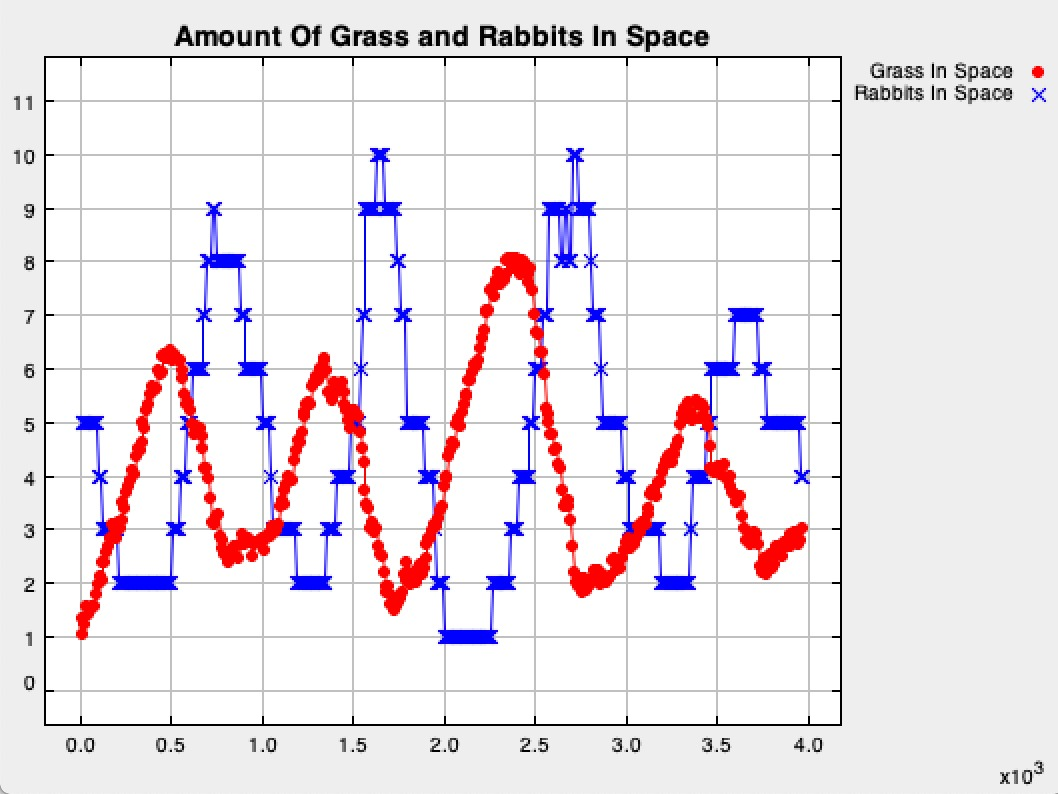
\includegraphics[width=0.5\columnwidth, frame]{Fig1.png}
        \caption{
                \label{fig:1}
                Blue: Number of living rabbits in the simulation space and Red: Amount of grass in the simulation space (scaled down to 2\% of actual value for visualisation)
        }
\end{figure}

% Elaborate on the observed results %

\subsection{Experiment 2: Stability}

\subsubsection{Setting}

After testing we have noticed two main types of stable situations: Grass Stable (Figure $2$a) and Rabbit Stable (Figure $2$b). \\
\indent If we consider the life cycle parameters as the base, we can obtain a Grass Stable situation by raising the \textit{grassGrowthRate} parameter (from 10 to 100 for example).\\
\indent However a Rabbit Stable situation is obtained by raising the \textit{minEnergy}, \textit{minEnergy} and therefore the \textit{birthThreshold} parameters (to 500, 1000 and 1500 respectively for example).
\indent Finally if we raise the \textit{birthThreshold} parameter (to 2000 for example) agents survive but in no particularly stable way.

\subsubsection{Observations}
% Elaborate on the observed results %

\begin{figure}[ht]
  \begin{subfigure}[t]{0.5\textwidth}
    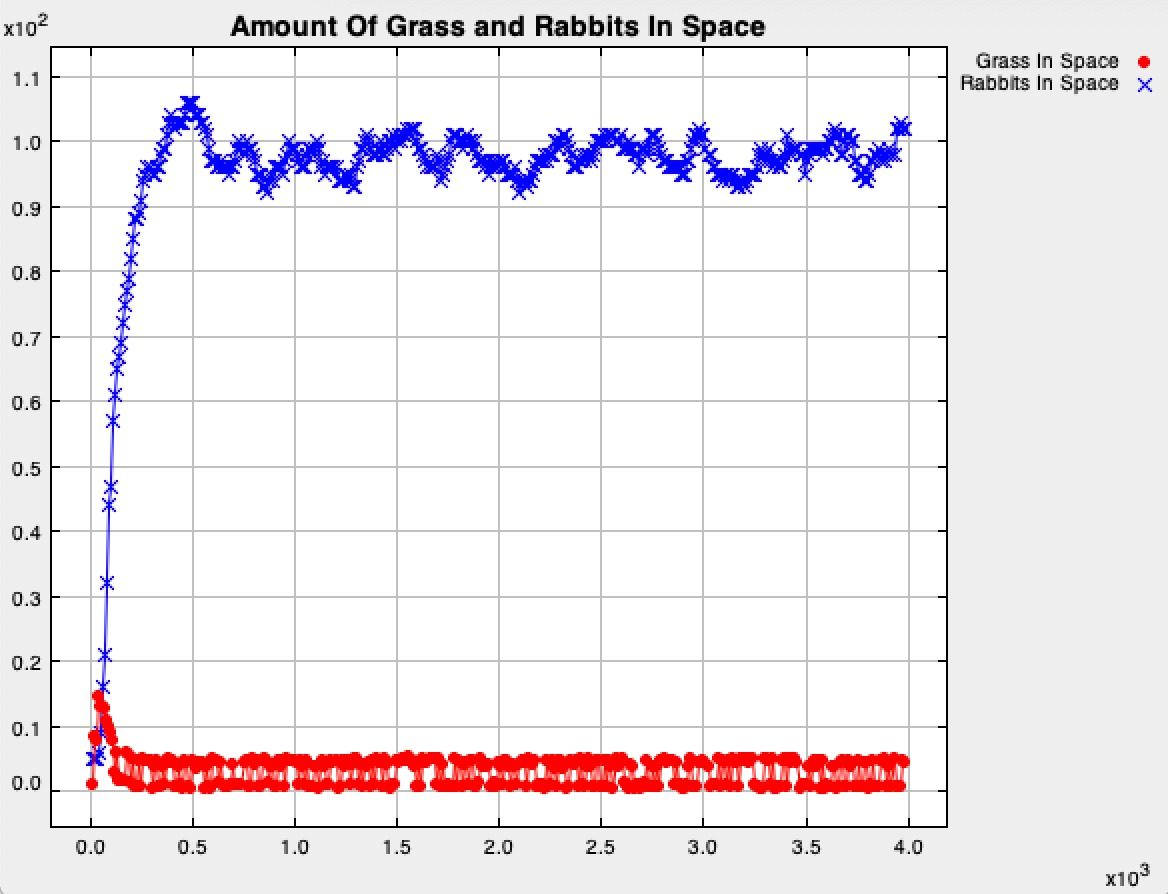
\includegraphics[width=\textwidth, frame]{Fig2a.png}
    \caption{Grass Stable Situation}
    \label{fig:2a}
  \end{subfigure}
  %
  \begin{subfigure}[t]{0.5\textwidth}
    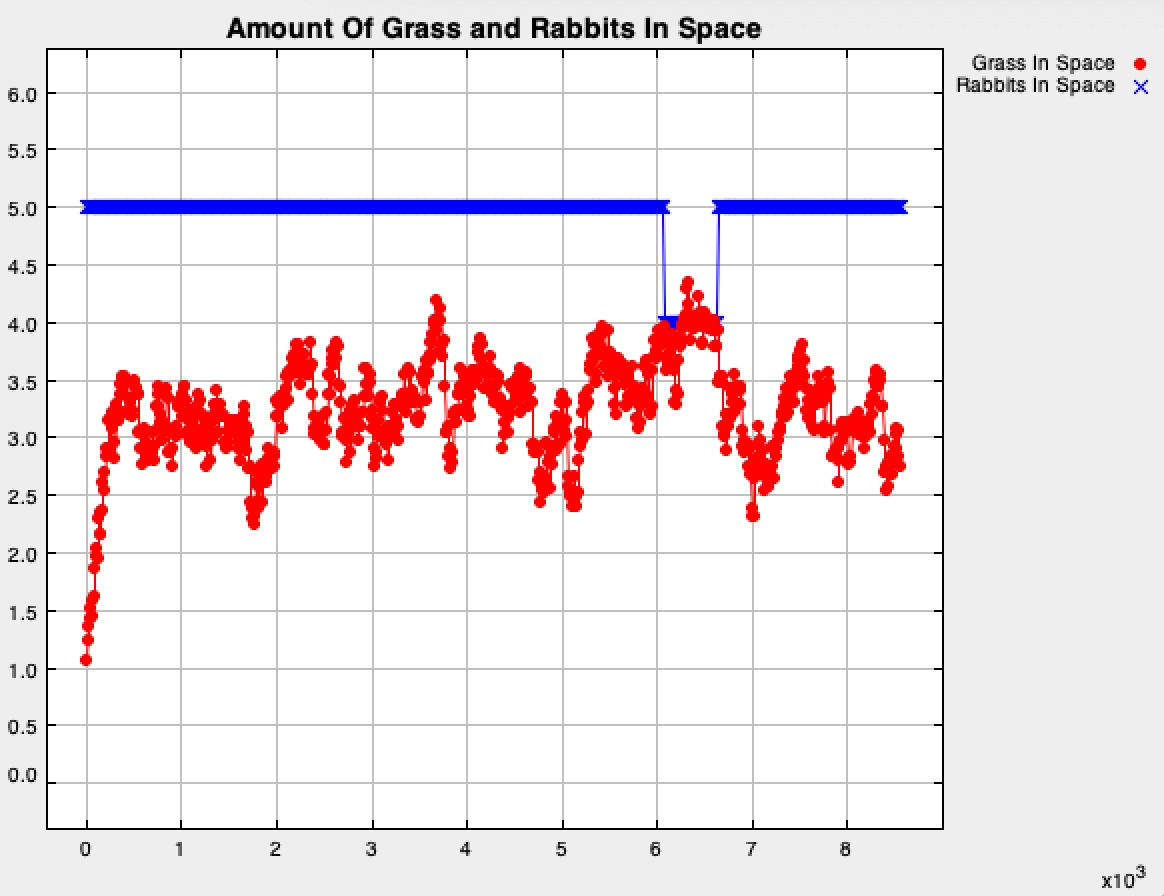
\includegraphics[width=\textwidth, frame]{Fig2b.png}
    \caption{Rabbit Stable Situation}
    \label{fig:2b}
  \end{subfigure}
  \label{fig:5}\caption{Blue: Number of living rabbits in the simulation space and Red: Amount of grass in the simulation space (scaled down to 2\% of actual value for visualisation)}
\end{figure}

In a Grass Stable situation, the amount of grass always stays constant, while the amount of rabbits is governed by the grass growth rate. Higher the growth rate, higher the amount of rabbits. \\
\indent In a Rabbit Stable Situation the grass varies around a certain level, but the amount of rabbits in the space stays constant with time. The rabbits have more energy to start and take longer to reproduce, but the food is sufficient for them to survive. Even if a rabbit dies, more food enables another one to reproduce keeping the number stable. The opposite also applies.

\subsection{Experiment 3: Extinction}

\subsubsection{Setting}

\indent Again, if we consider the life cycle parameters as the base, extinction is observed in a few situations. By lowering the \textit{birthThreshold} to the \textit{maxEnergy} limit, by reducing the \textit{grassGrowthRate} parameter, by raising the initial amount of rabbits \textit{numInitRabbits} or the initial amount of grass \textit{numInitGrass}. 

\subsubsection{Observations}
% Elaborate on the observed results %

If we lower the textit{birthThreshold} to the \textit{maxEnergy} limit rabbits will reproduce very fast, overpopulating the space. All the grass is eaten and the rabbits have nothing left. We can compensate this by raising the \textit{grassGrowthRate}. \\
\indent However if we reduce the \textit{grassGrowthRate}, the grass has no time to grow before it is eaten by the rabbits. They then starve, similarly to the previous situation. \\
\indent Raising \textit{numInitRabbits} or \textit{numInitGrass} without touching bthe other parameters have a similar effect. With a high amount of starting rabbits, all the grass is eaten fast, energy is wasted and the rabbits die. With a high initial amount of grass, the rabbits have the opportunity to reproduce fast, overpopulating the space as explained previously.

\end{document}
